\chapter{Ergebnisse und Ausblick}
\section{Erreichte Funktionalitäten}

In Abbildung \ref{fig:startseite} ist die Startseite der WebApp zu sehen. Sie bietet eine Übersicht über die wichtigsten Funktionen und ermöglicht den schnellen Zugriff auf den Stundenplan, Notizen, Kalender und Einstellungen. Die Startseite ist so gestaltet, dass sie eine klare Navigation und eine ansprechende Benutzeroberfläche bietet.\newline
\begin{figure}[H]
  \centering
  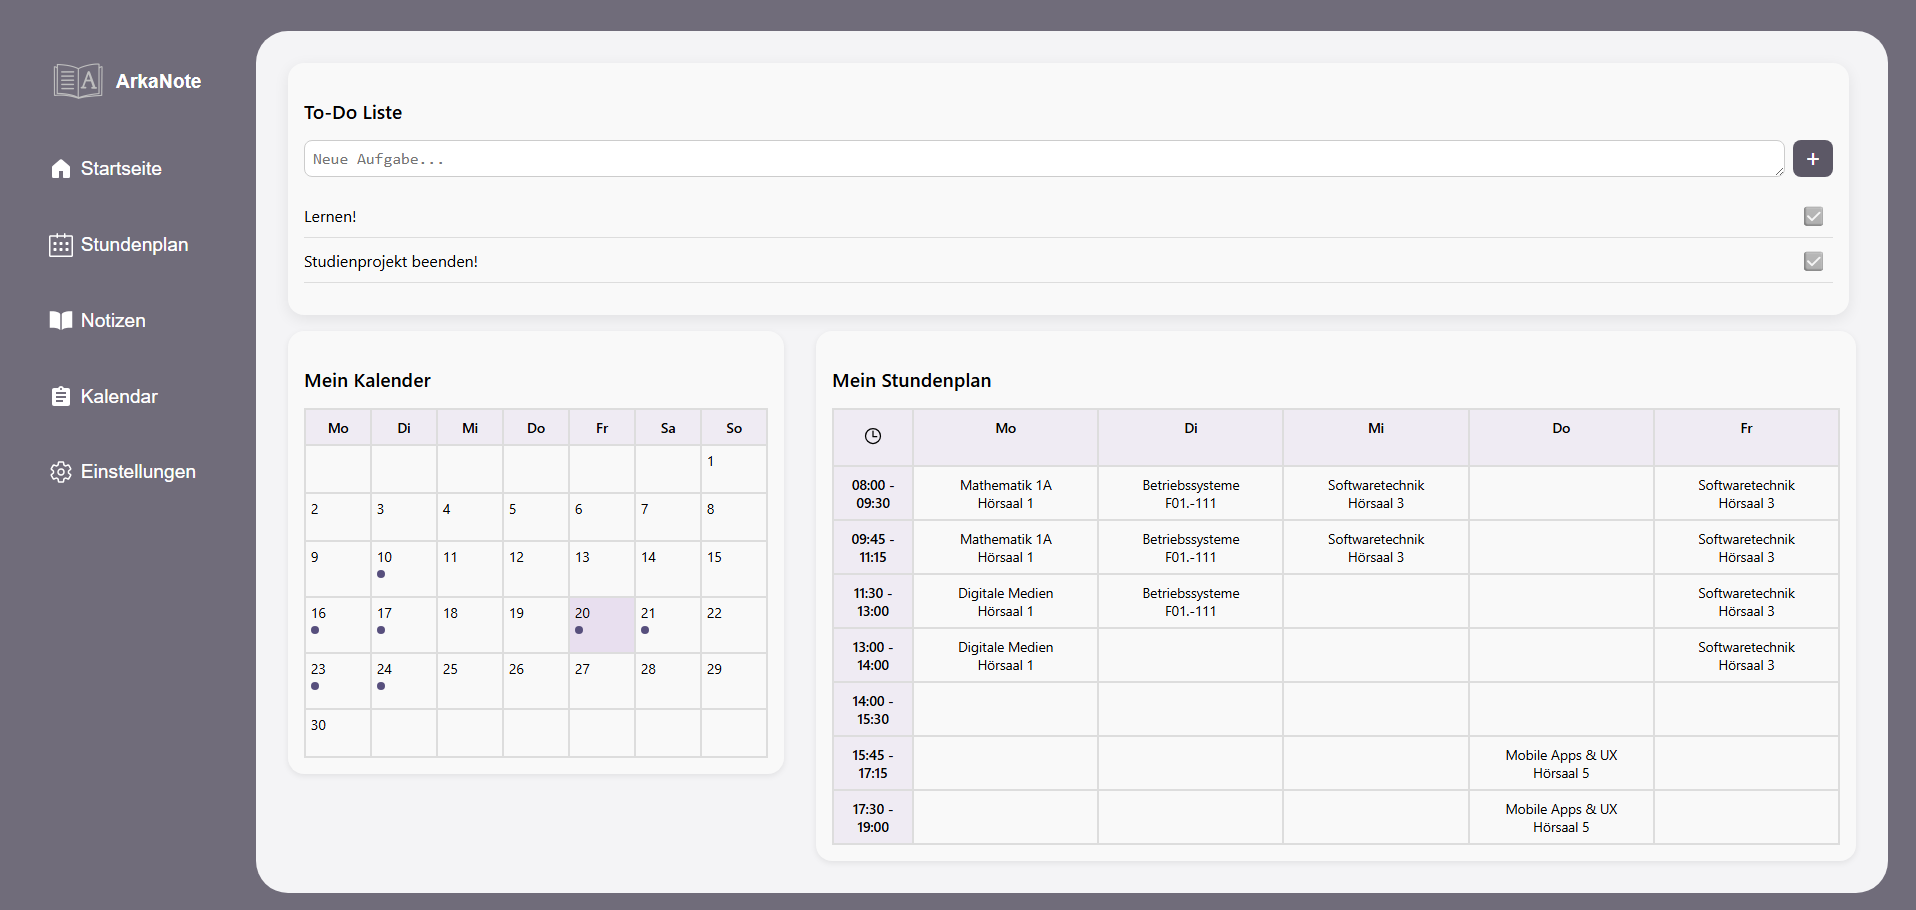
\includegraphics[width=1\textwidth]{./images/startseite.png}
  \caption{Startseite}
  \label{fig:startseite}
\end{figure}

Die WebApp ermöglicht es den Nutzer:innen, Vorlesungen zu verwalten und in ihren Stundenplan einzutragen. In Abbildung \ref{fig:stundenplan} ist der Stundenplan zu sehen, der eine visuelle Darstellung der Vorlesungen bietet. Nutzer:innen können neue Vorlesungen hinzufügen, wie in Abbildung \ref{fig:neue-vorlesungen} gezeigt, und diese dann in ihren Stundenplan eintragen (Abbildung \ref{fig:stundenplan-vorlesung}).\newline
\begin{figure}[H]
  \centering
  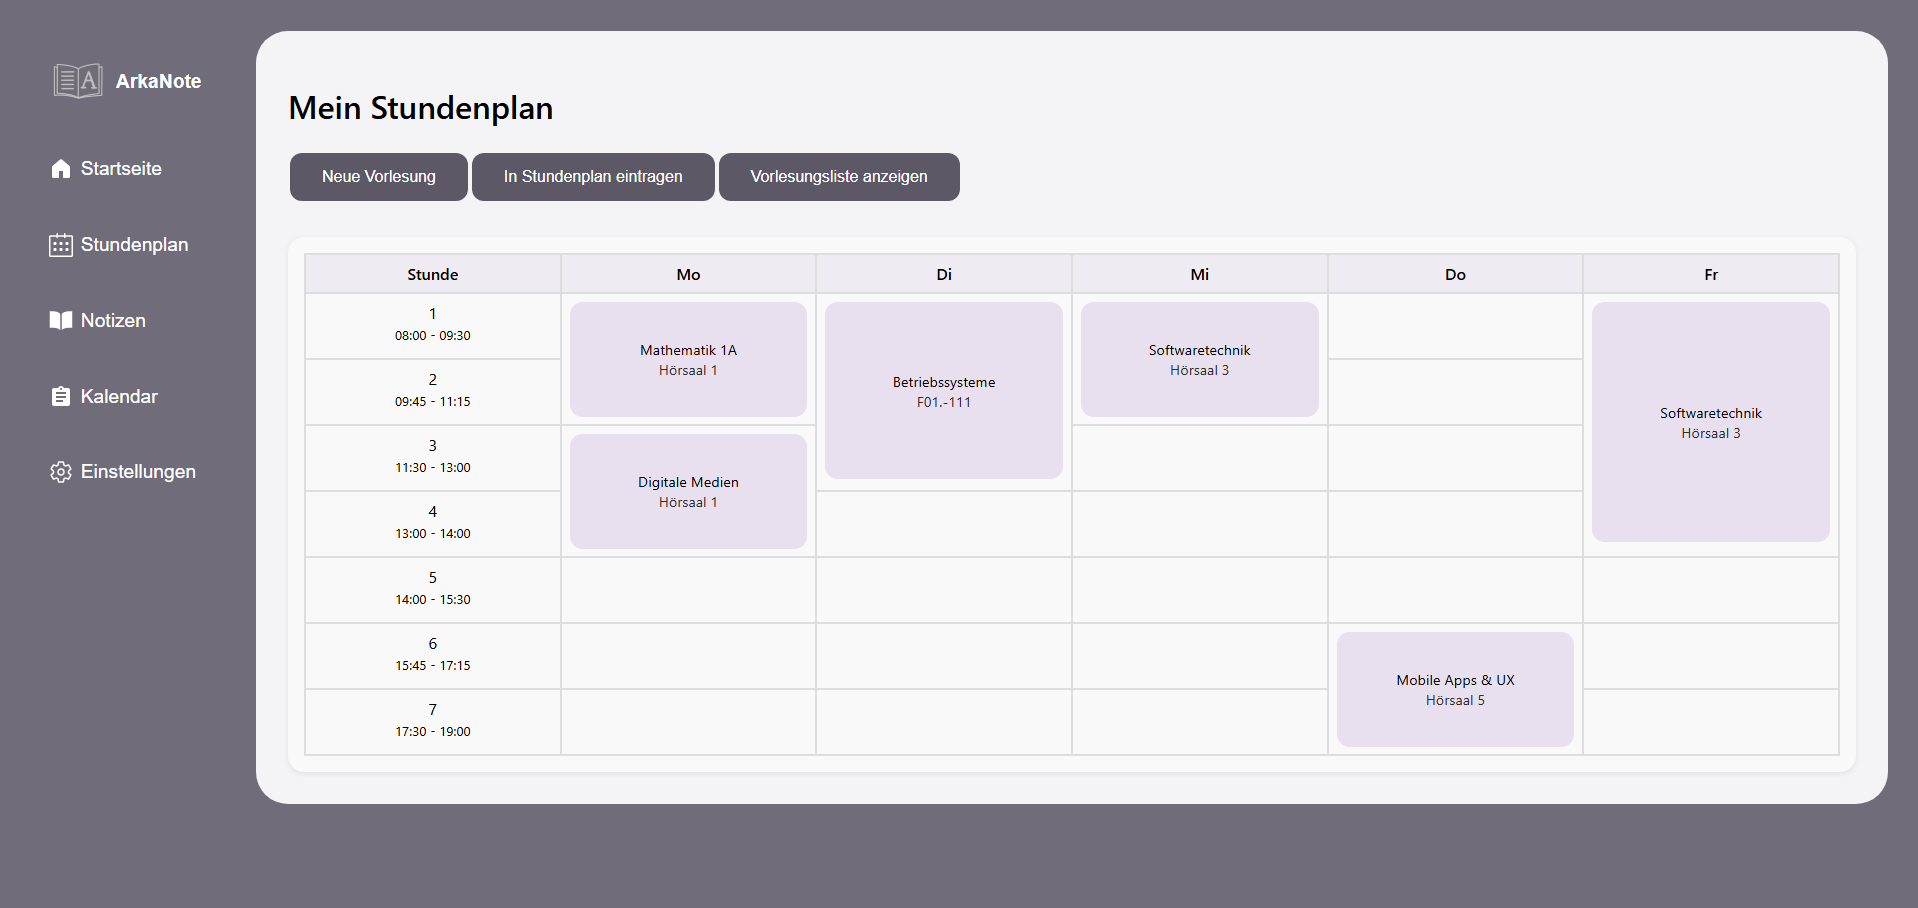
\includegraphics[width=1\textwidth]{./images/stundenplan.png}
  \caption{Stundenplan}
  \label{fig:stundenplan}
\end{figure}

\begin{figure}[H]
  \centering
  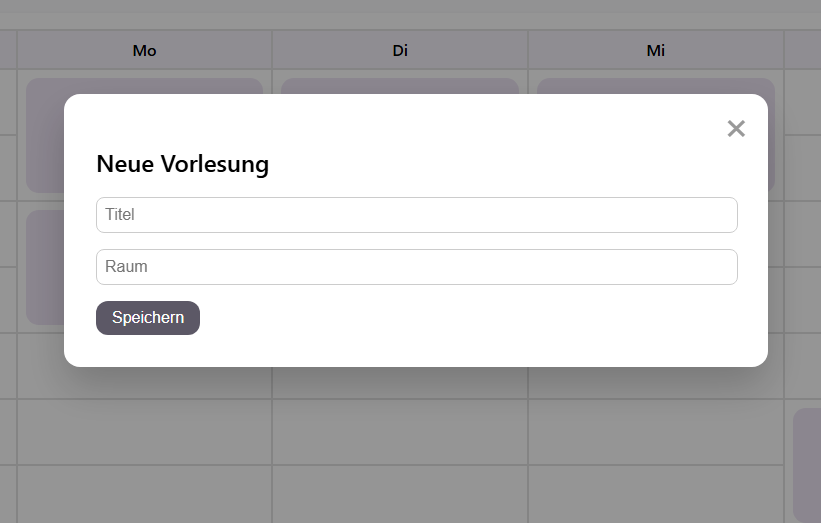
\includegraphics[width=1\textwidth]{./images/stundenplan-neuevorlesung.png}
  \caption{Neue Vorlesung hinzufügen}
  \label{fig:neue-vorlesungen}
\end{figure}

\begin{figure}[H]
  \centering
  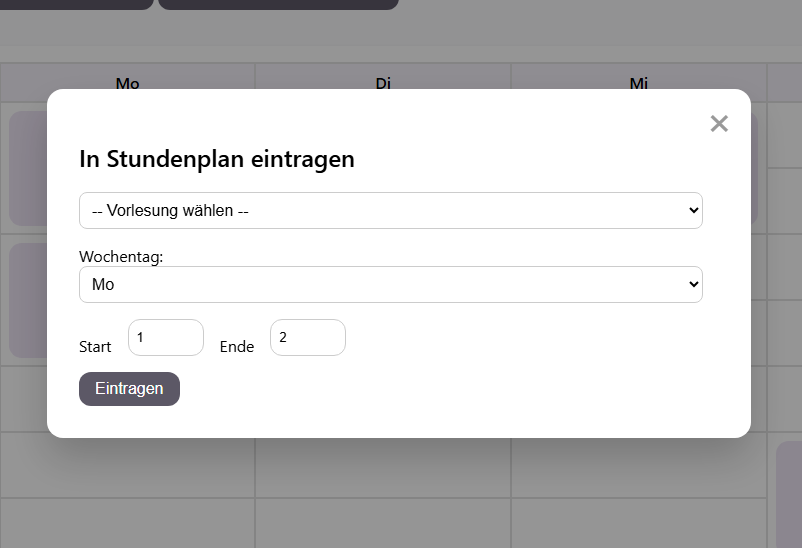
\includegraphics[width=1\textwidth]{./images/stundenplan-instundenplan.png}
  \caption{Vorlesung in den Stundenplan eintragen}
  \label{fig:stundenplan-vorlesung}
\end{figure}

Abbildung \ref{fig:stundenplan-vorlesungen} zeigt die Vorlesungsliste, in der alle verfügbaren Vorlesungen aufgelistet sind. Nutzer:innen können aus dieser Liste Vorlesungen löschen.
\begin{figure}[H]
  \centering
  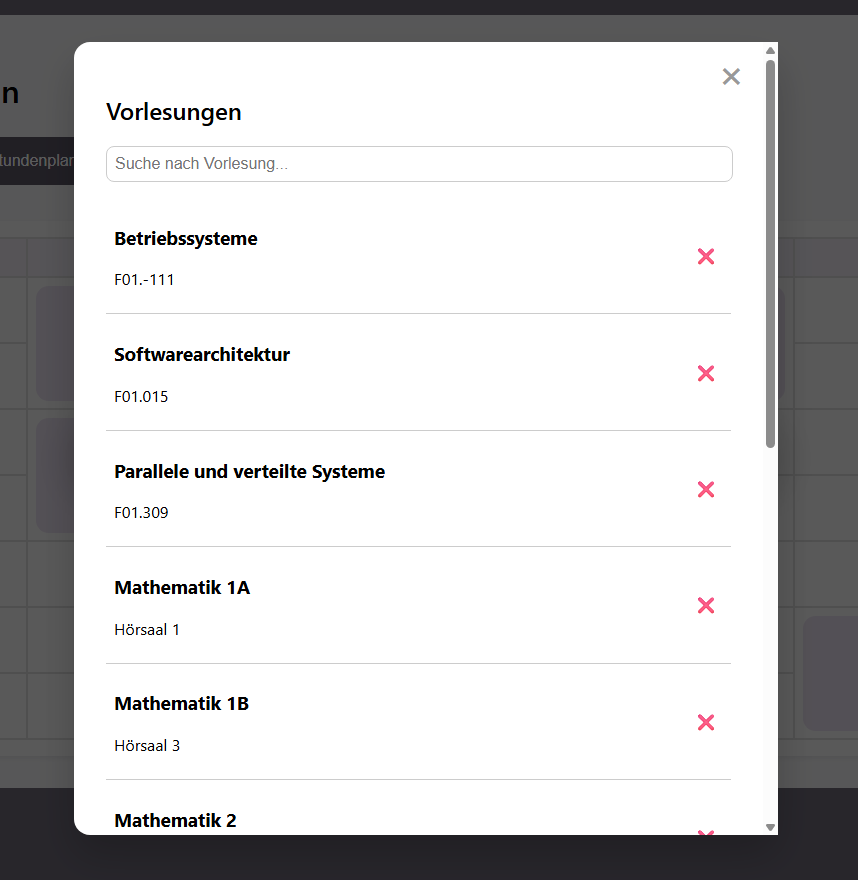
\includegraphics[width=1\textwidth]{./images/stundenplan-vorlesungsliste.png}
  \caption{Vorlesungsliste}
  \label{fig:stundenplan-vorlesungen}
\end{figure}

Die Web App bietet auch eine Notizfunktion, die es den Nutzer:innen ermöglicht, Notizen zu Vorlesungen zu erstellen und zu verwalten. In Abbildung \ref{fig:notizen} sind die Notizen und Lernmaterialien zu sehen, die hochgeladen und kategorisiert werden können. Nutzer:innen können Notizen zu spezifischen Vorlesungen hinzufügen und diese nach Bedarf organisieren.\newline
\begin{figure}[H]
  \centering
  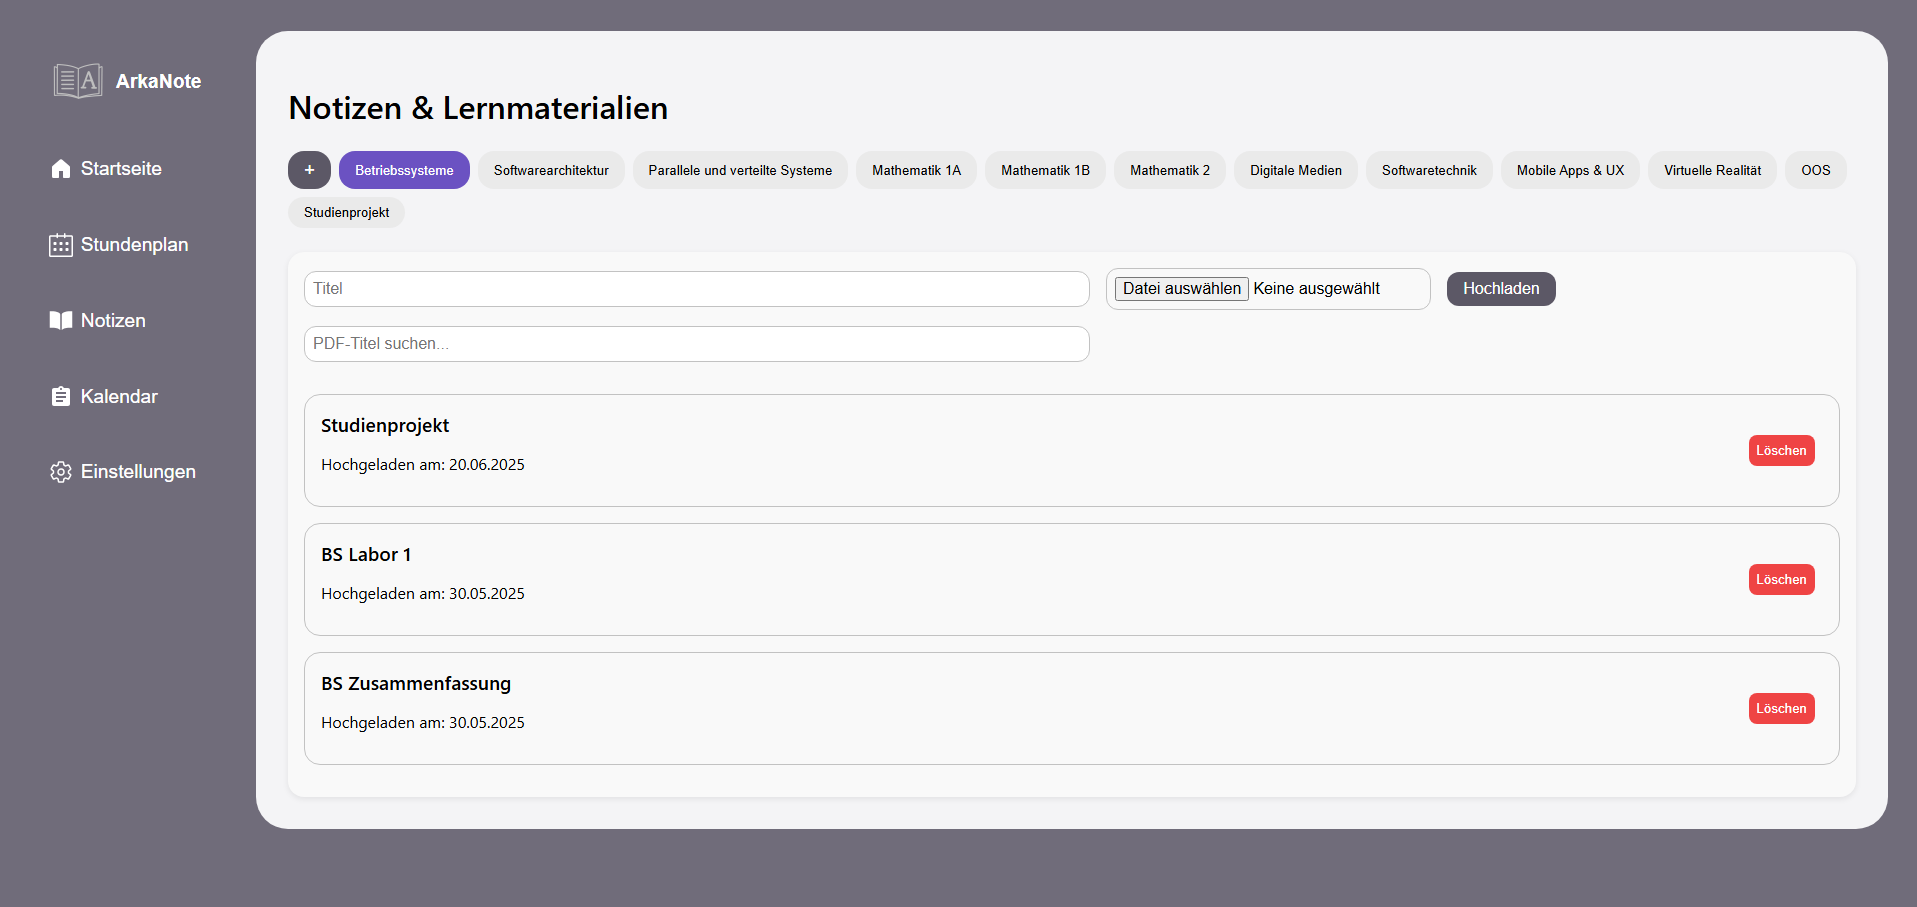
\includegraphics[width=1\textwidth]{./images/notizen.png}
  \caption{Notizen und Lernmaterialien}
  \label{fig:notizen}
\end{figure}

Die Kalenderfunktion der Web App ermöglicht es den Nutzer:innen, Termine und Fristen zu verwalten. In Abbildung \ref{fig:kalender} ist der Kalender zu sehen, in dem Nutzer:innen Ereignisse hinzufügen können, wie in Abbildung \ref{fig:kalender-ereignis} gezeigt. Diese Funktionalität ist besonders nützlich, um wichtige Termine im Blick zu behalten und eine bessere Organisation des Studienalltags zu ermöglichen.\newline
\begin{figure}[H]
  \centering
  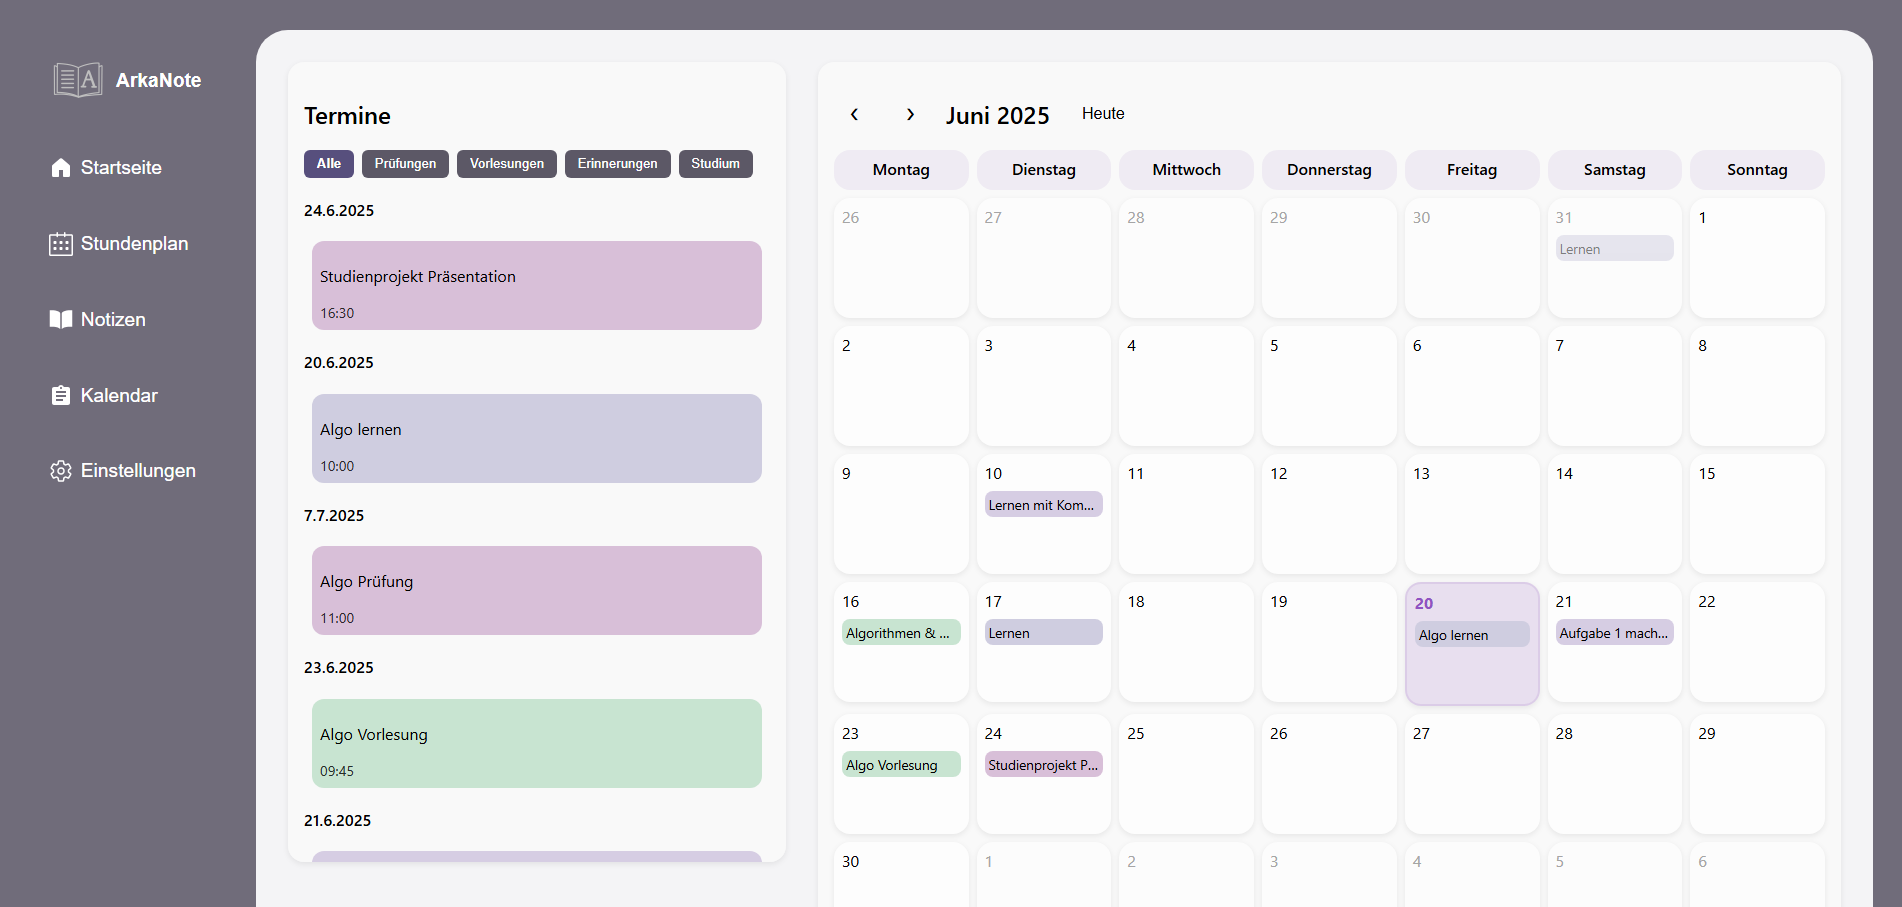
\includegraphics[width=1\textwidth]{./images/kalender.png}
  \caption{Kalender}
  \label{fig:kalender}
\end{figure}

\begin{figure}[H]
  \centering
  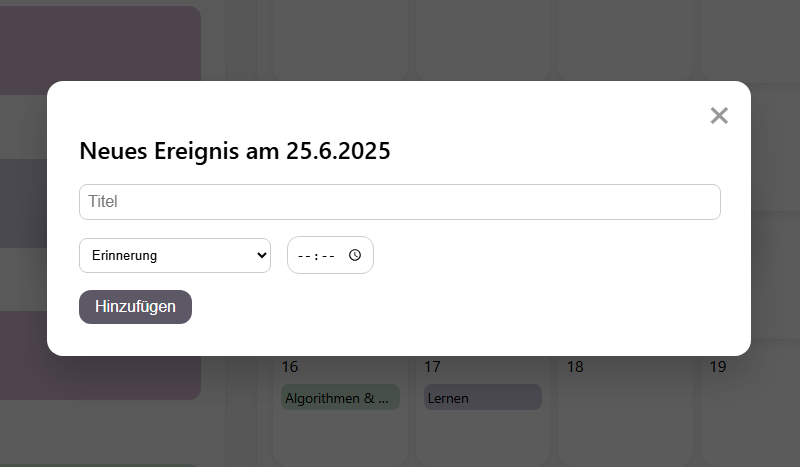
\includegraphics[width=1\textwidth]{./images/kalender-ereignis.png}
  \caption{Kalenderereignis hinzufügen}
  \label{fig:kalender-ereignis}
\end{figure}

Abbildung \ref{fig:einstellungen} zeigt die Einstellungen der Web App, in denen Nutzer:innen ihre persönlichen Daten verwalten und das Design der Anwendung anpassen können. \newline
\begin{figure}[H]
  \centering
  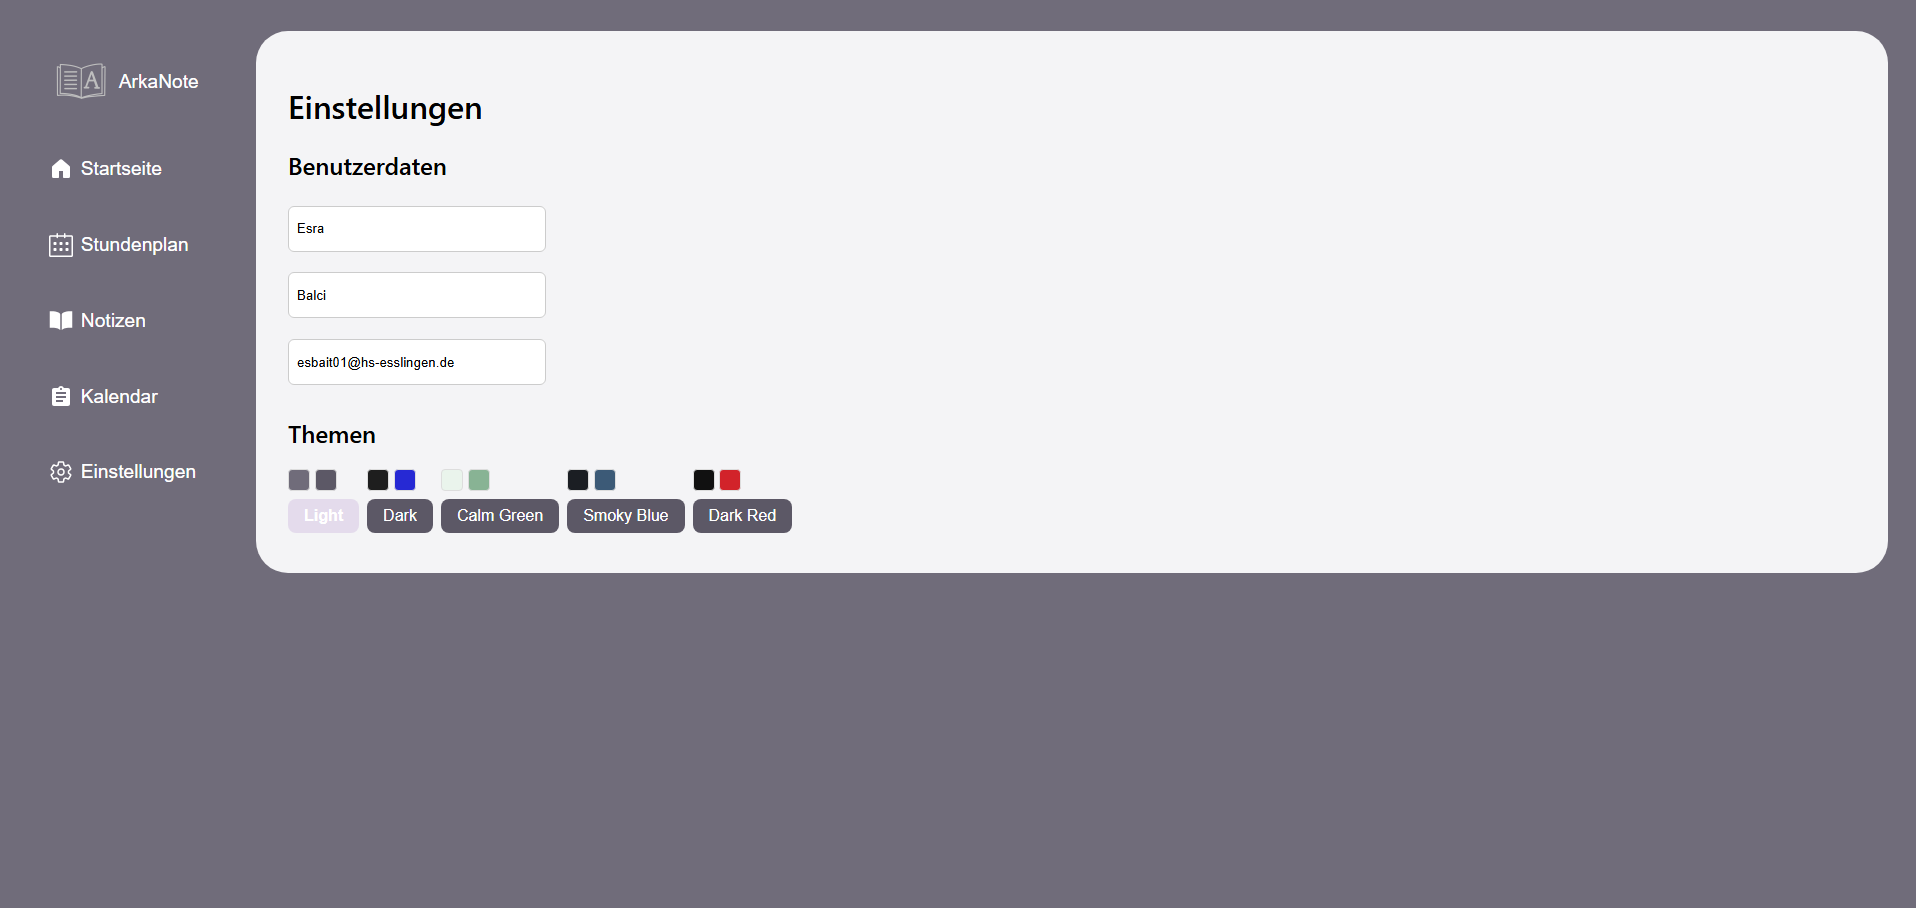
\includegraphics[width=1\textwidth]{./images/einstellungen.png}
  \caption{Einstellungen}
  \label{fig:einstellungen}
\end{figure}

Die Web App bietet verschiedene Design-Themes, die den Nutzer:innen eine individuelle Anpassung ermöglichen. In den Abbildungen \ref{fig:startseite-dark}, \ref{fig:kalender-dark}, \ref{fig:startseite-green}, \ref{fig:kalender-green}, \ref{fig:startseite-blue}, \ref{fig:kalender-blue}, \ref{fig:startseite-red} und \ref{fig:kalender-red} sind die verschiedenen Themes zu sehen, die den Nutzer:innen zur Verfügung stehen.\newline
\begin{figure}[H]
  \centering
  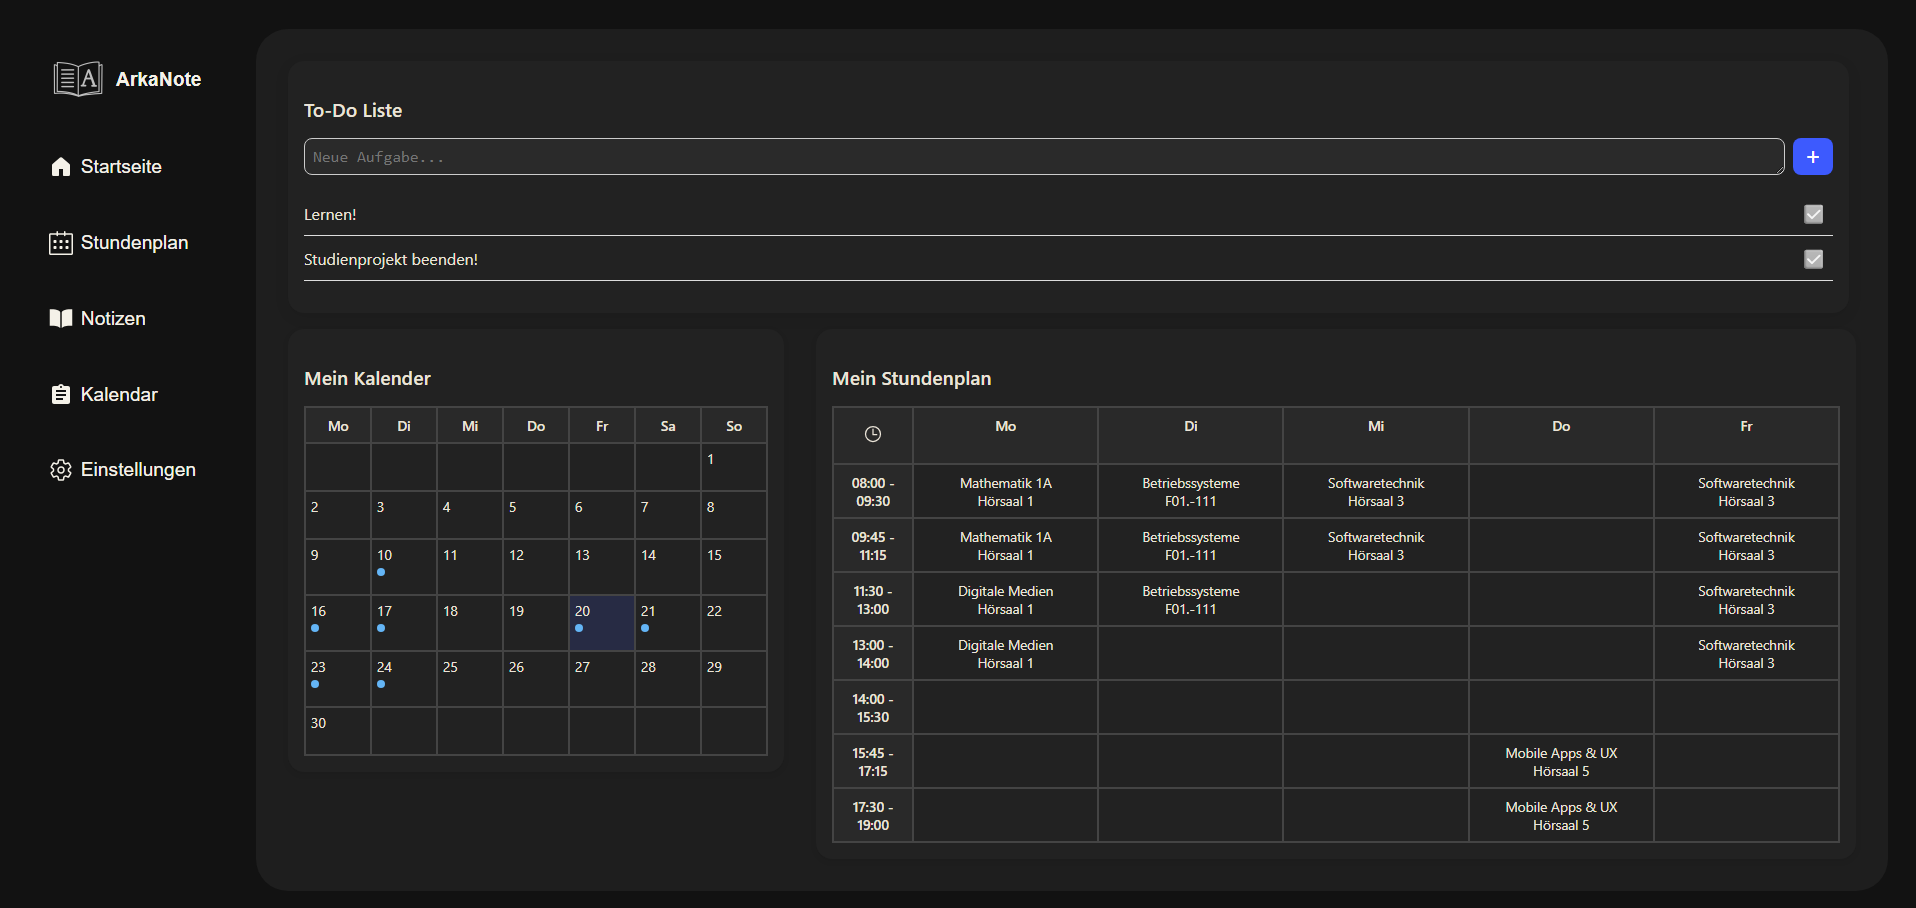
\includegraphics[width=1\textwidth]{./images/startseite-dark.png}
  \caption{Startseite im Dark Theme}
  \label{fig:startseite-dark}
\end{figure}

\begin{figure}[H]
  \centering
  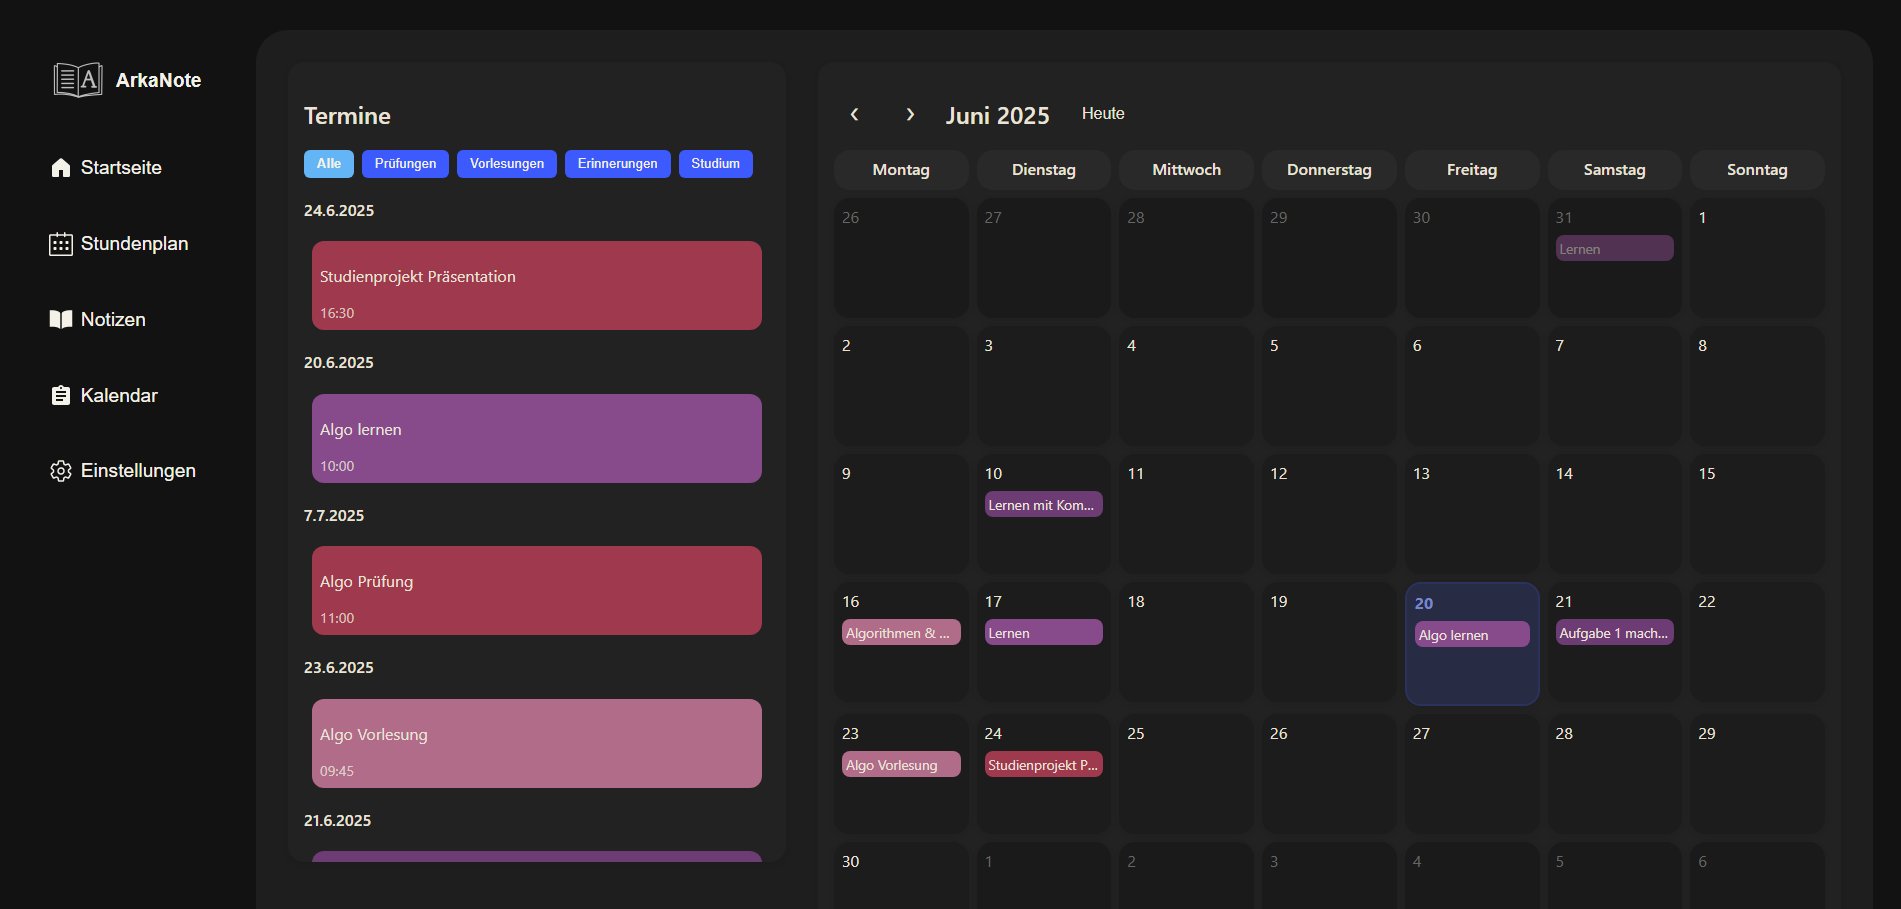
\includegraphics[width=1\textwidth]{./images/kalender-dark.png}
  \caption{Kalender im Dark Theme}
  \label{fig:kalender-dark}
\end{figure}

\begin{figure}[H]
  \centering
  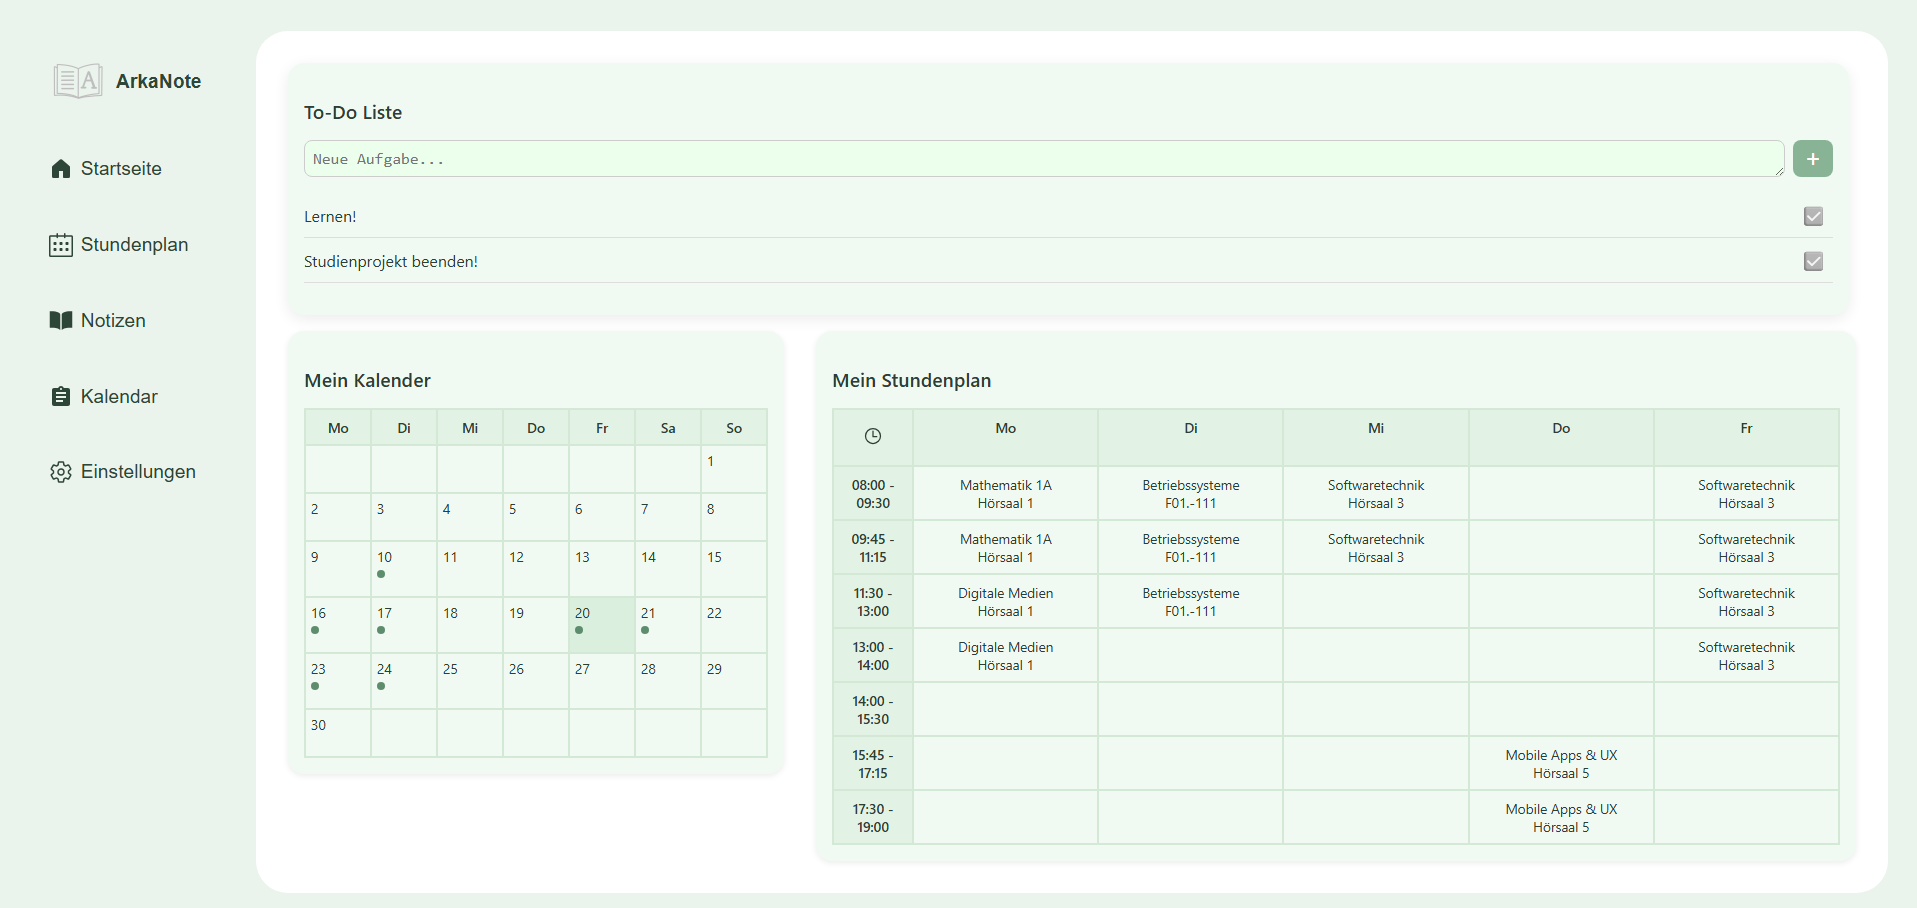
\includegraphics[width=1\textwidth]{./images/startseite-green.png}
  \caption{Startseite im Calm Green Theme}
  \label{fig:startseite-green}
\end{figure}

\begin{figure}[H]
  \centering
  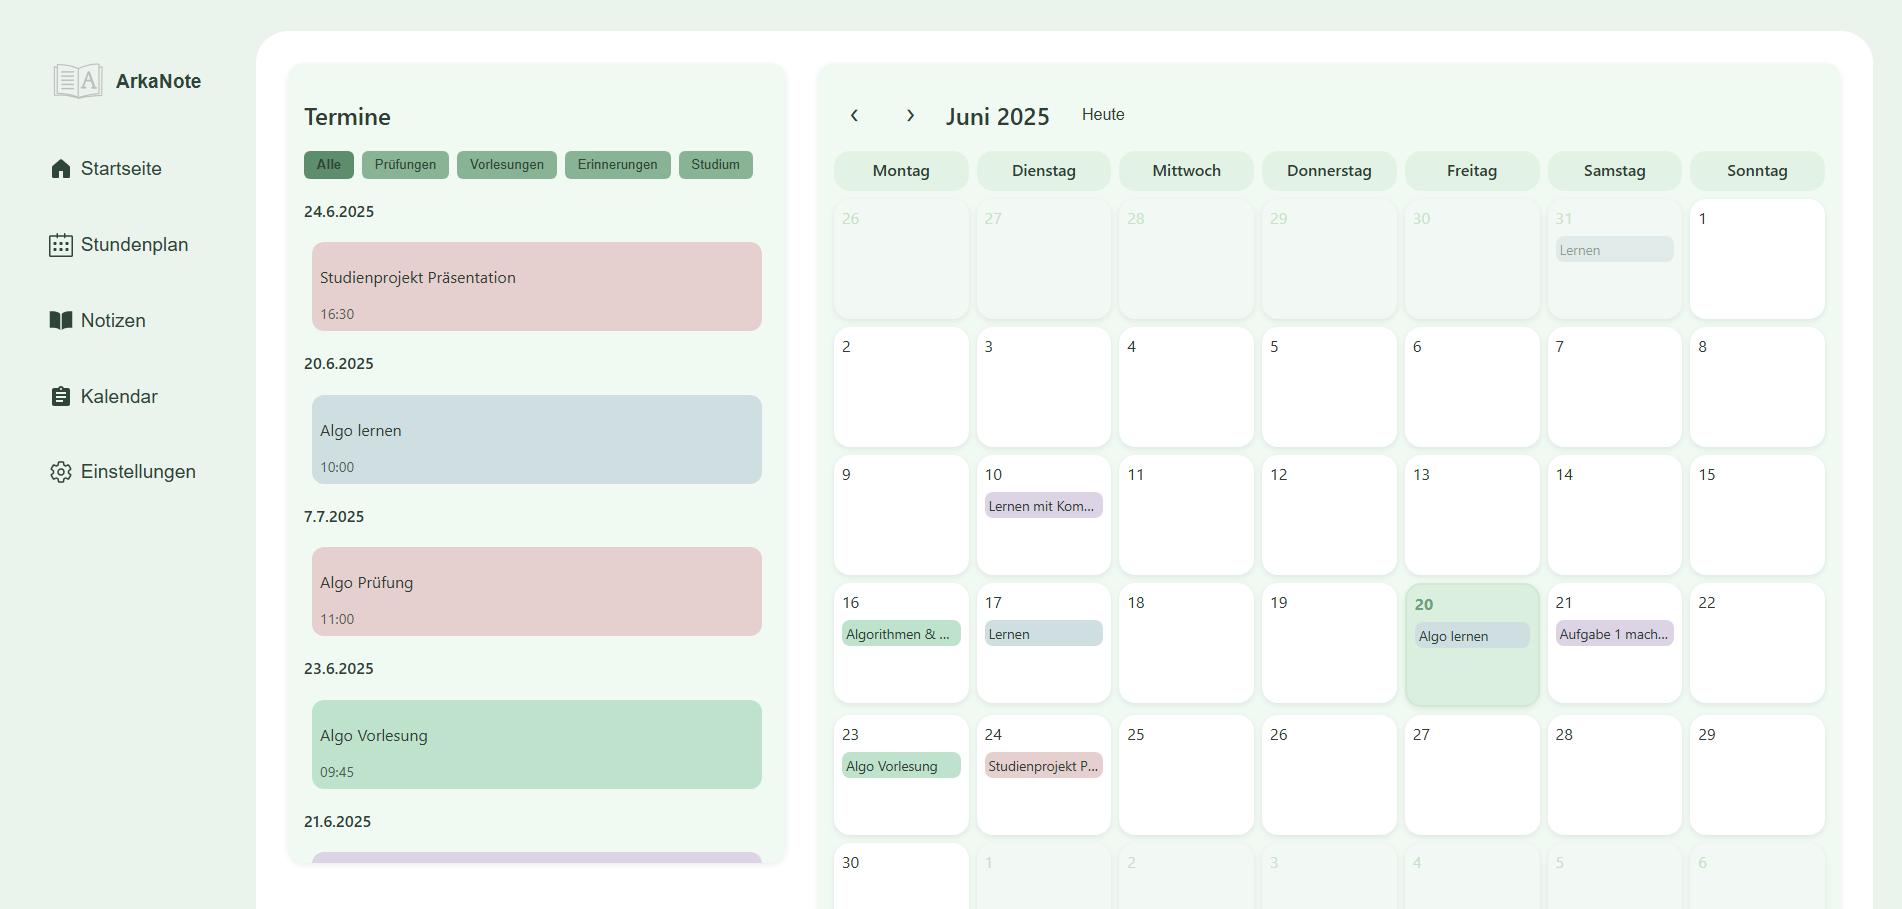
\includegraphics[width=1\textwidth]{./images/kalender-green.png}
  \caption{Kalender im Calm Green Theme}
  \label{fig:kalender-green}
\end{figure}

\begin{figure}[H]
  \centering
  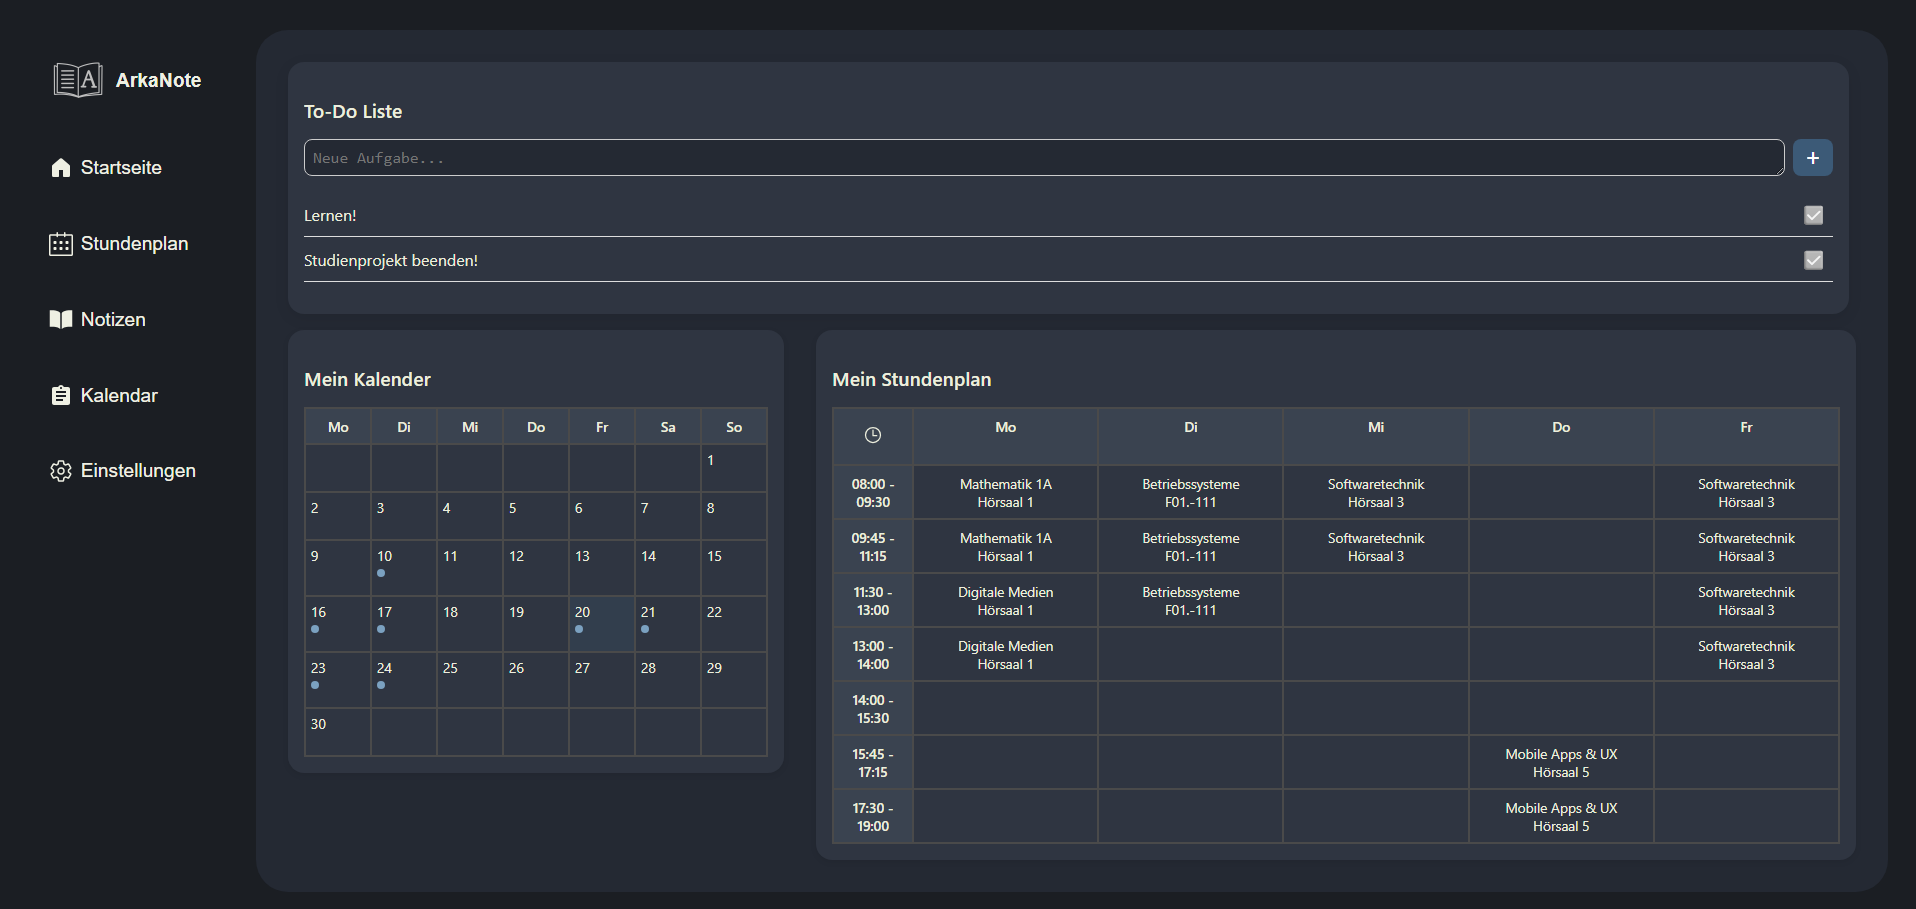
\includegraphics[width=1\textwidth]{./images/startseite-blue.png}
  \caption{Startseite im Smoky Blue Theme}
  \label{fig:startseite-blue}
\end{figure}

\begin{figure}[H]
  \centering
  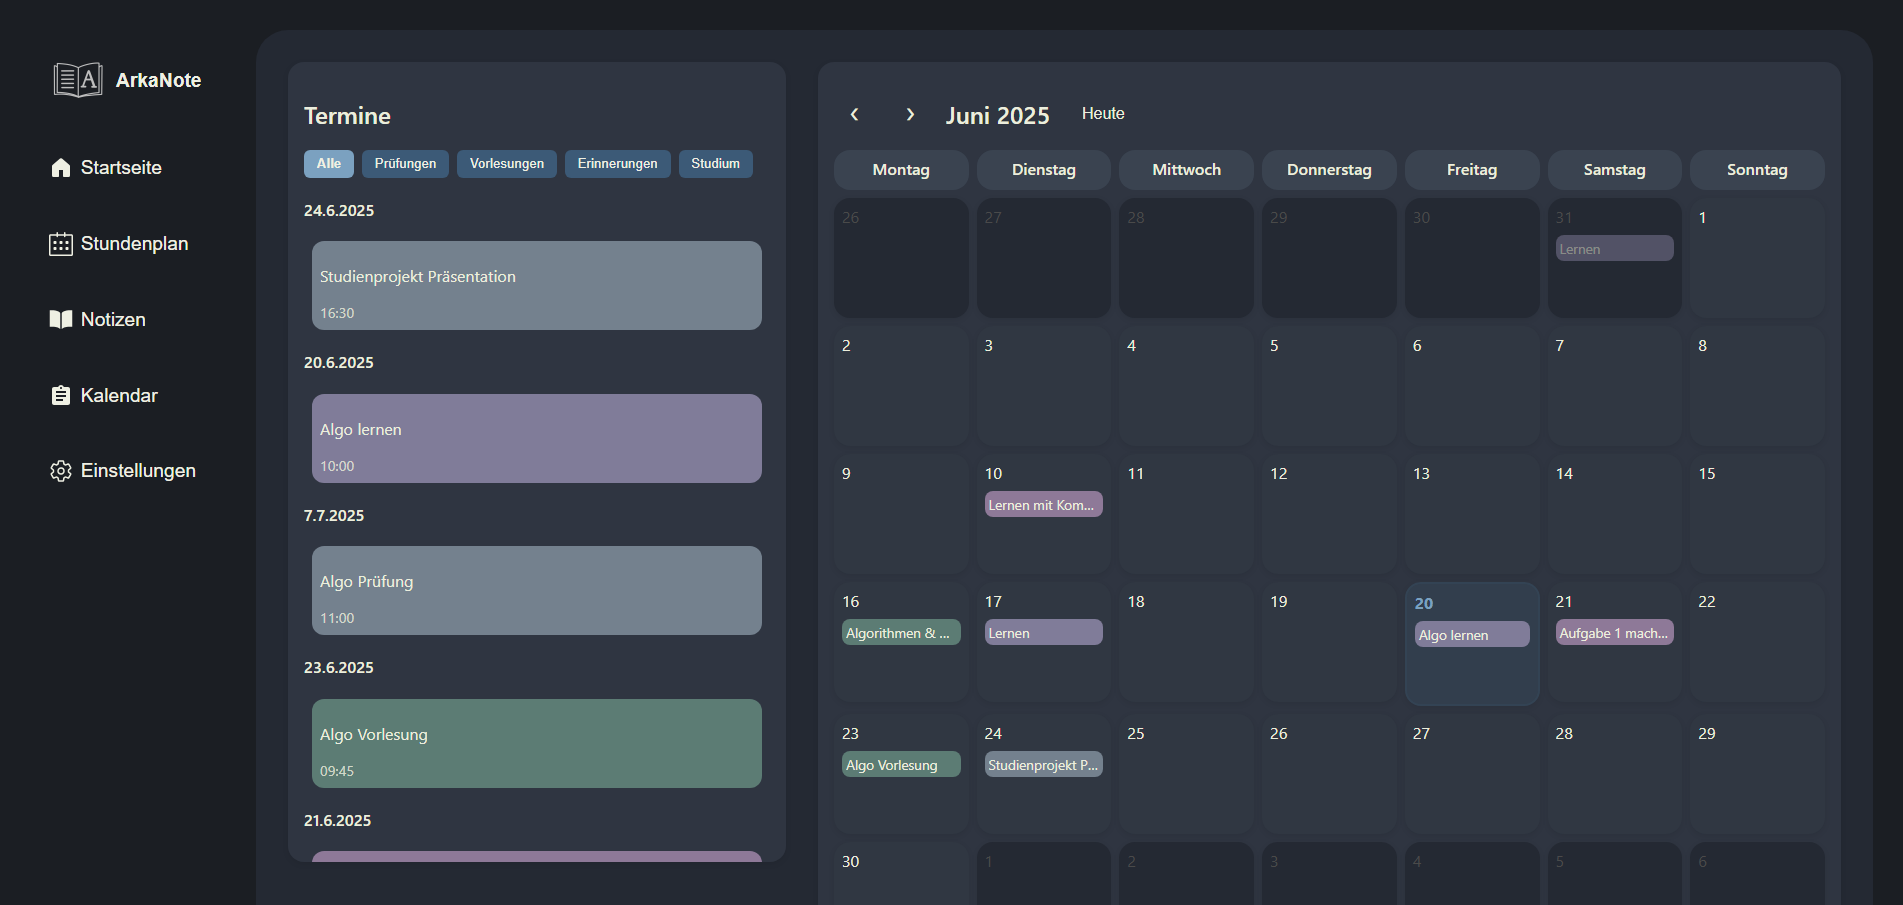
\includegraphics[width=1\textwidth]{./images/kalender-blue.png}
  \caption{Kalender im Smoky Blue Theme}
  \label{fig:kalender-blue}
\end{figure}

\begin{figure}[H]
  \centering
  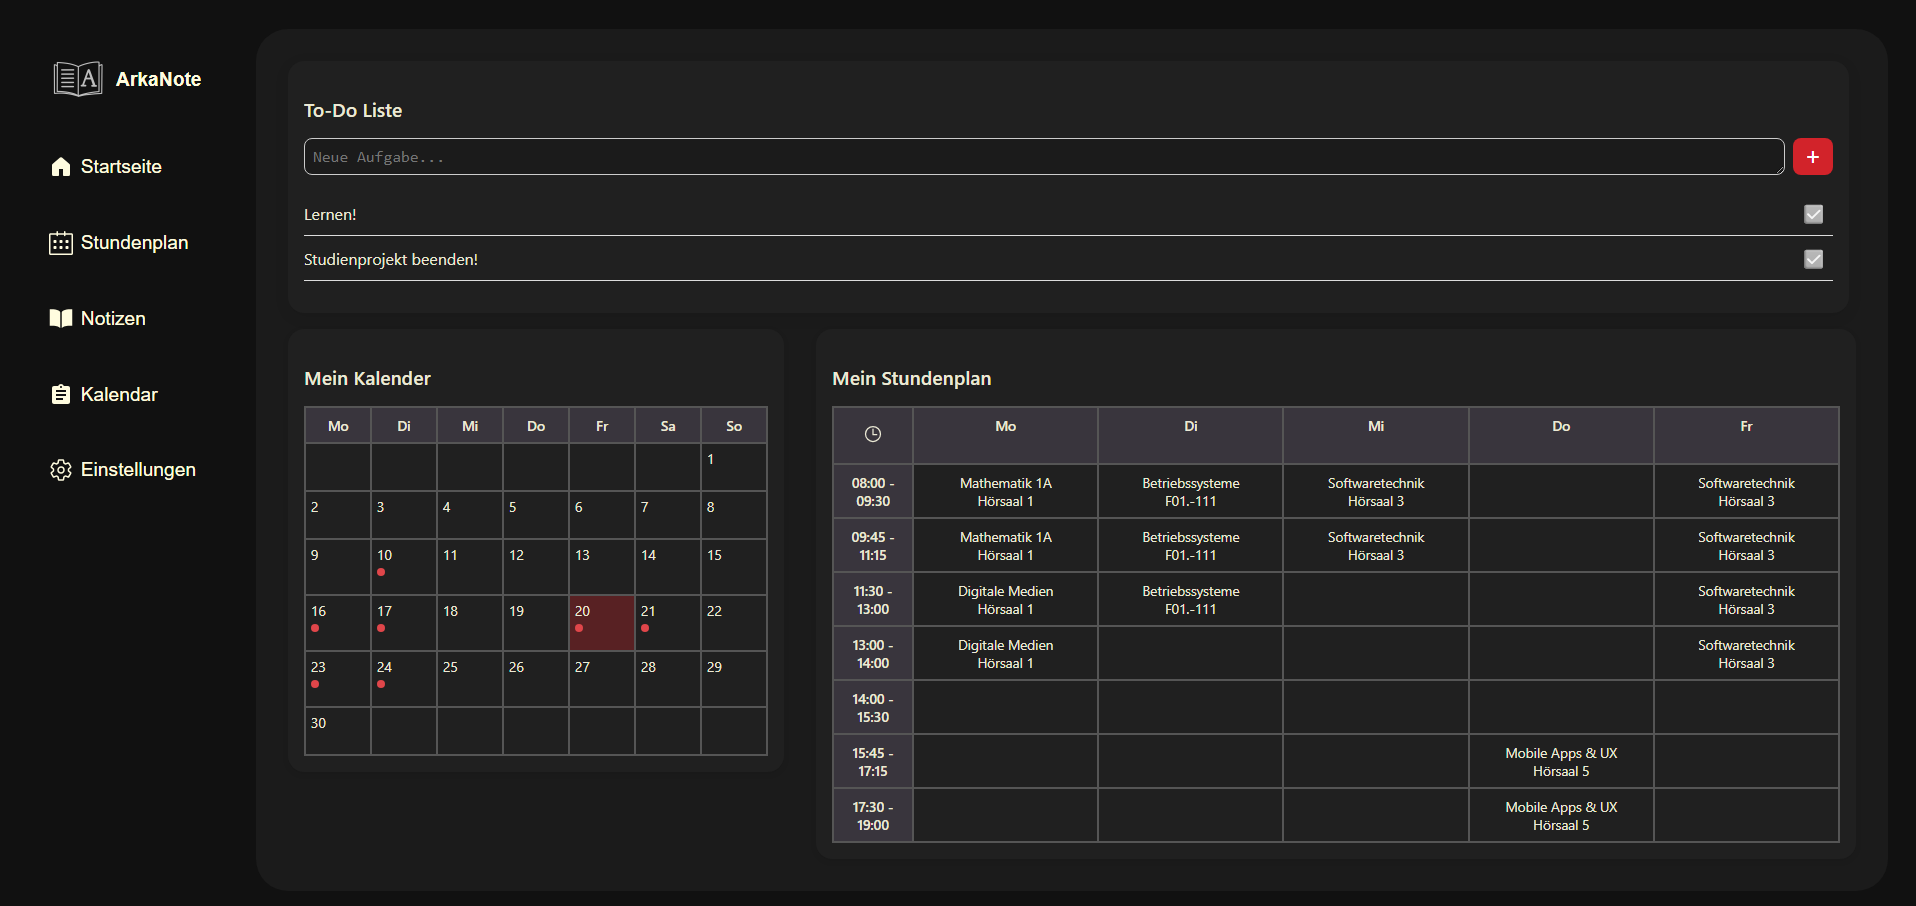
\includegraphics[width=1\textwidth]{./images/startseite-red.png}
  \caption{Startseite im Dark Red Theme}
  \label{fig:startseite-red}
\end{figure}

\begin{figure}[H]
  \centering
  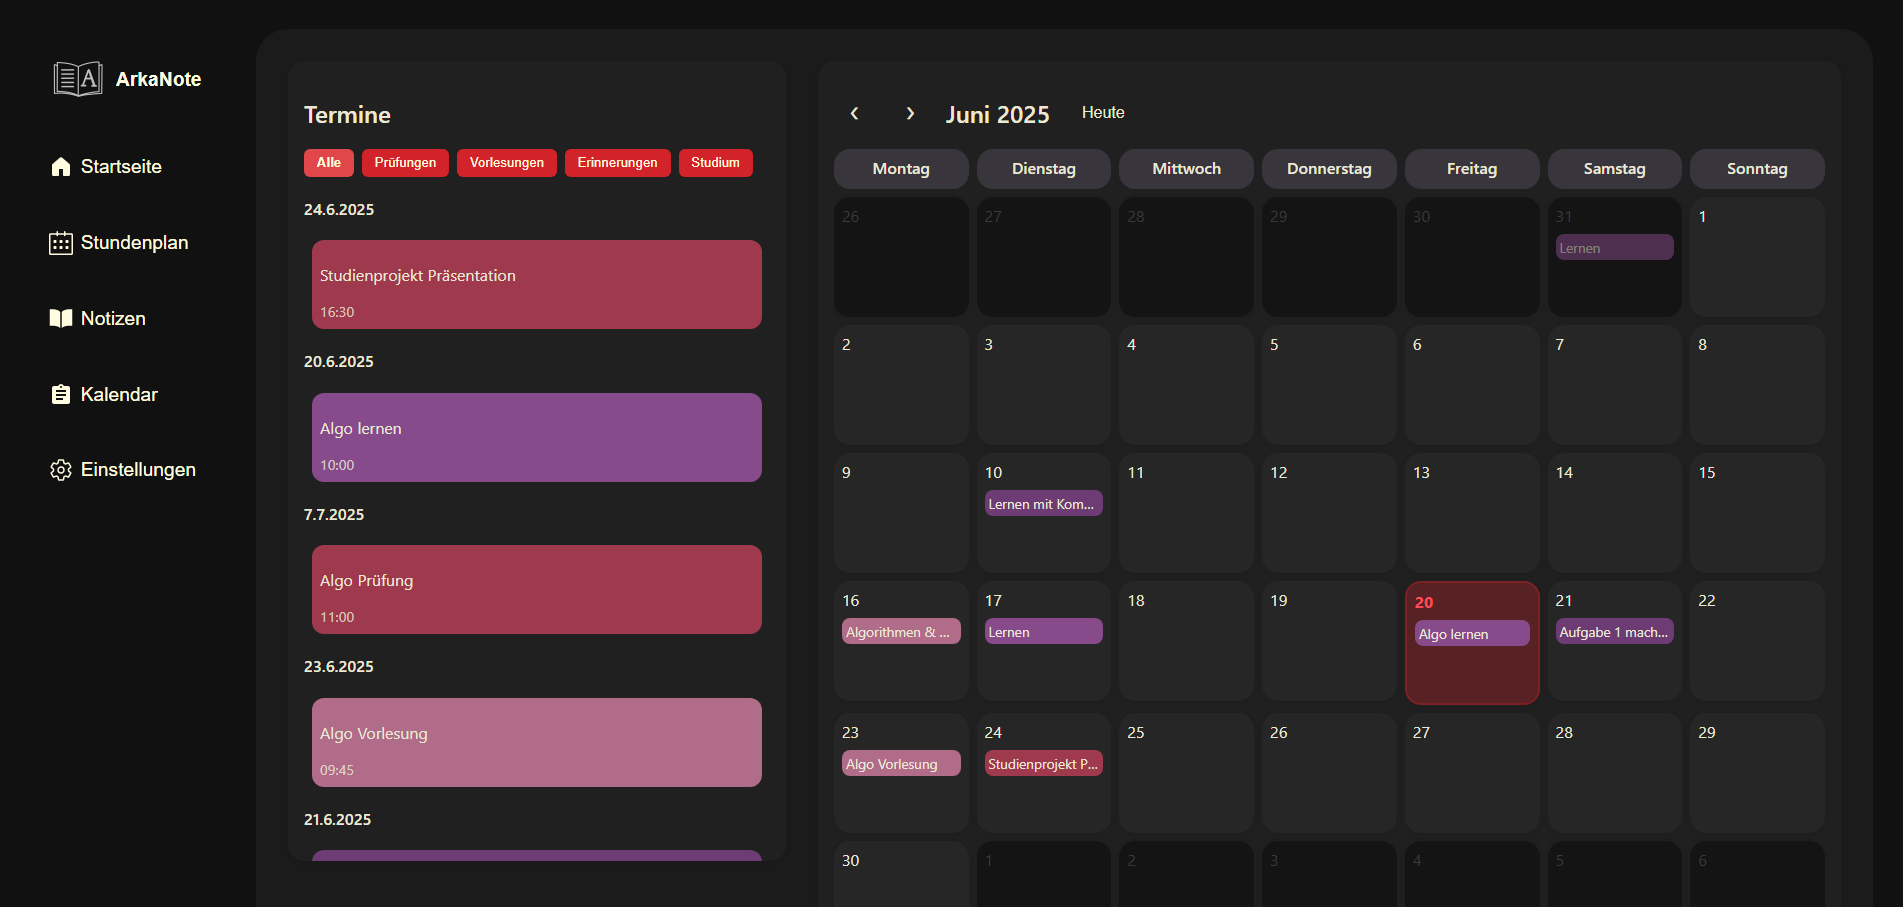
\includegraphics[width=1\textwidth]{./images/kalender-red.png}
  \caption{Kalender im Dark Red Theme}
  \label{fig:kalender-red}
\end{figure}

\section{Vergleich zu bestehenden Lösungen}
\begin{table}[H]
\centering
\scriptsize % kleinere Schriftgröße für bessere Lesbarkeit
\renewcommand{\arraystretch}{1.3} % etwas mehr Zeilenhöhe
\begin{tabularx}{\textwidth}{|p{3cm}|p{2.3cm}|p{2.5cm}|p{2.5cm}|p{2.5cm}|}
\hline
\textbf{Kriterium / Tool} & \textbf{Projekt} & \textbf{Moodle} & \textbf{Google Kalender} & \textbf{Notion} \\
\hline
Zielgruppe & Studierende, selbstorganisiert & Hochschulen, Lehrende + Studis & Allgemein, breites Publikum & Teams, Selbstorganisation \\
\hline
Stundenplan-Funktion & Visuell und interaktiv & Nicht enthalten & Nur Ereignisse & Manuell möglich \\
\hline
Kalender & Mit Deadlines und Kategorien & Mit Farbcodes + Kategorien & Eingeschränkt, wenig UX & Sehr leistungsfähig, aber unstrukturiert \\
\hline
Notizen mit Tags & Uploads & PDF-Upload + Tagging & Nur in Foren/Dateien & Sehr stark (Rich Content) \\
\hline
Offline-Funktion (PWA) & Nein & Nein & Nur mit Google Workspace & Nur mit App \\
\hline
Gebrauchstauglichkeit (UI) & Modern, Studierendenfokus & Veraltet, überladen & Klar und bekannt & Flexibel, aber komplex \\
\hline
Plattformunabhängigkeit & Web + App & Web + App & Web + App & Web + App \\
\hline
Open Source / Anpassbar & Ja (Eigenentwicklung möglich) & Teilweise & Nein & Nein \\
\hline
Integration in Lernumgebung & Manuell über Nutzung & Hochschulweit integriert & Nur externe Anbindung & Nur Copy/Paste \\
\hline
\end{tabularx}
\caption{Vergleich vom Projekt mit bestehenden Tools für studentisches Selbstmanagement}
\label{tab:toolvergleich}
\end{table}



\section{Offene Punkte und mögliche Erweiterungen}
Die entwickelte Web App erfüllt grundlegende Anforderungen an ein digitales Selbstorganisationswerkzeug, weist jedoch in ihrer aktuellen Version noch einige funktionale und technische Lücken auf, die in zukünftigen Entwicklungsschritten adressiert werden sollten.\newline 
Derzeit besteht keine Möglichkeit zur geräteübergreifenden Synchronisation von Daten. Dies bedeutet dass die Nutzung auf ein einzelnes Gerät beschränkt bleibt. Eine logische Weiterentwicklung stellt die Einführung eines cloudbasierten Backends mit Benutzerverwaltung dar.\newline 
Zudem fehlen Push-Benachrichtigungen, die die Nutzer:innen aktiv an bevorstehende Termine und Fristen erinnern könnten. Die Integration solcher Erinnerungsfunktionen würde den Nutzwert der App im Studienalltag deutlich steigern, insbesondere in Verbindung mit der Kalenderfunktion.\newline 
Neben der technischen Weiterentwicklung bestehen auch funktionale Erweiterungspotenziale. So wäre beispielsweise die Unterstützung von Gruppenfunktionen denkbar, bei der Studierende gemeinsame Notizen verwalten oder Termine in Lerngruppen organisieren können. Dies würde die Web App auch für kollaborative Lernszenarien attraktiver machen.\newline 
Langfristig ließe sich die Anwendung zudem durch den Einsatz Künstlicher Intelligenz erweitern. Möglich wären beispielsweise automatische Zusammenfassungen von Notizen oder intelligente Vorschläge für die Terminplanung auf Basis individueller Lernmuster. Diese Erweiterungen könnten nicht nur die Effizienz der Web App steigern, sondern auch den indiviuellen Lernprozess der Studierenden nachhaltig fördern.